
\documentclass[12pt,a4paper,twoside,openany]{book}

% Modern fonts and typographical packages
\usepackage{fontspec}         % Allows font customization (XeLaTeX/LuaLaTeX)
\usepackage{microtype}        % Enhances typographical output
\usepackage{lmodern}          % Latin Modern fonts (fallback for math mode)
\usepackage{ebgaramond}       % Elegant Garamond font for text
\usepackage{titlesec}         % Customize section titles
\usepackage{fancyhdr}         % Custom headers and footers
\usepackage{wrapfig}
\usepackage{tcolorbox}
\usepackage{caption}
\setlength{\headheight}{14.5pt}  % Adjust to avoid fancyhdr warning
\addtolength{\topmargin}{-2.5pt}

% Page and layout settings
\usepackage[a4paper,margin=2.5cm]{geometry}   % Adjust margins
\usepackage{multicol}         % For multiple column layouts
\usepackage{parskip}          % Space between paragraphs
\usepackage{setspace}         % Line spacing
\usepackage{graphicx}         % For including images
\usepackage{enumitem}
\graphicspath{{graphics/}}
\usepackage{xcolor}           % Text and background color
\usepackage{booktabs}         % Professional-quality tables
\usepackage{hyperref}         % Hyperlinks in the PDF
\usepackage{subfiles}
\hypersetup{
    colorlinks=true,
    linkcolor=blue,
    filecolor=magenta,      
    urlcolor=cyan,
}

% Custom headers
\pagestyle{fancy}
\fancyhf{}
\fancyhead[LE,RO]{\thepage}
\fancyhead[LO]{\nouppercase{\leftmark}}
\fancyhead[RE]{\nouppercase{\rightmark}}

% Chapter title customization
\titleformat{\chapter}[hang]
  {\normalfont\Huge\bfseries}{\thechapter}{2em}{}
  
% Section title customization
\titleformat{\section}[block]{\Large\bfseries}{\thesection}{1em}{}

% Color scheme (adjust for aesthetic)
\definecolor{fateblue}{HTML}{00539C} % Fate Core blue
\definecolor{chaptergray}{gray}{0.2}

% Custom title page
\newcommand{\booktitle}{Fate Core: Asterion}
\newcommand{\authorname}{Racek et. al. }

\newcommand{\asp}[1]{\textbf{\textit{#1}}}


\newcommand{\prekonani}{%
  \begin{wrapfigure}{l}{1cm}  
    \vspace{10pt}  
    
\includegraphics[width=1.5cm]{prekonani-ikona}
  \end{wrapfigure}
  \leavevmode\ignorespaces  % To ensure proper alignment with the text
}

\newcommand{\vytvoreni}{%
  \begin{wrapfigure}{l}{1cm}  
    \vspace{10pt}  
    
\includegraphics[width=1.5cm]{vytvoreni-ikona}
  \end{wrapfigure}
  \leavevmode\ignorespaces  % To ensure proper alignment with the text
}


\newcommand{\utok}{%
  \begin{wrapfigure}{l}{1cm}  
    \vspace{10pt}  
    
\includegraphics[width=1.5cm]{utok-ikona}
  \end{wrapfigure}
  \leavevmode\ignorespaces  % To ensure proper alignment with the text
}

\newcommand{\obrana}{%
  \begin{wrapfigure}{l}{1cm}  
    \vspace{10pt}  
    
\includegraphics[width=1.5cm]{obrana-ikona}
  \end{wrapfigure}
  \leavevmode\ignorespaces  % To ensure proper alignment with the text
}


\newenvironment{akce}
{ % Begin definition
  \begin{itemize}[label={}]
}
{ % End definition
  \end{itemize}
}


\newcommand{\iconitem}[2]{%
\item \raisebox{-0.5\height}{\includegraphics[width=1.5cm]{#1}} \ #2%
  
}



\begin{document}

% Title page
\begin{titlepage}
    \centering
    {\Huge\textbf{\booktitle}}\\[1.5cm]
    {\Large by \textit{\authorname}}\\[2cm]
    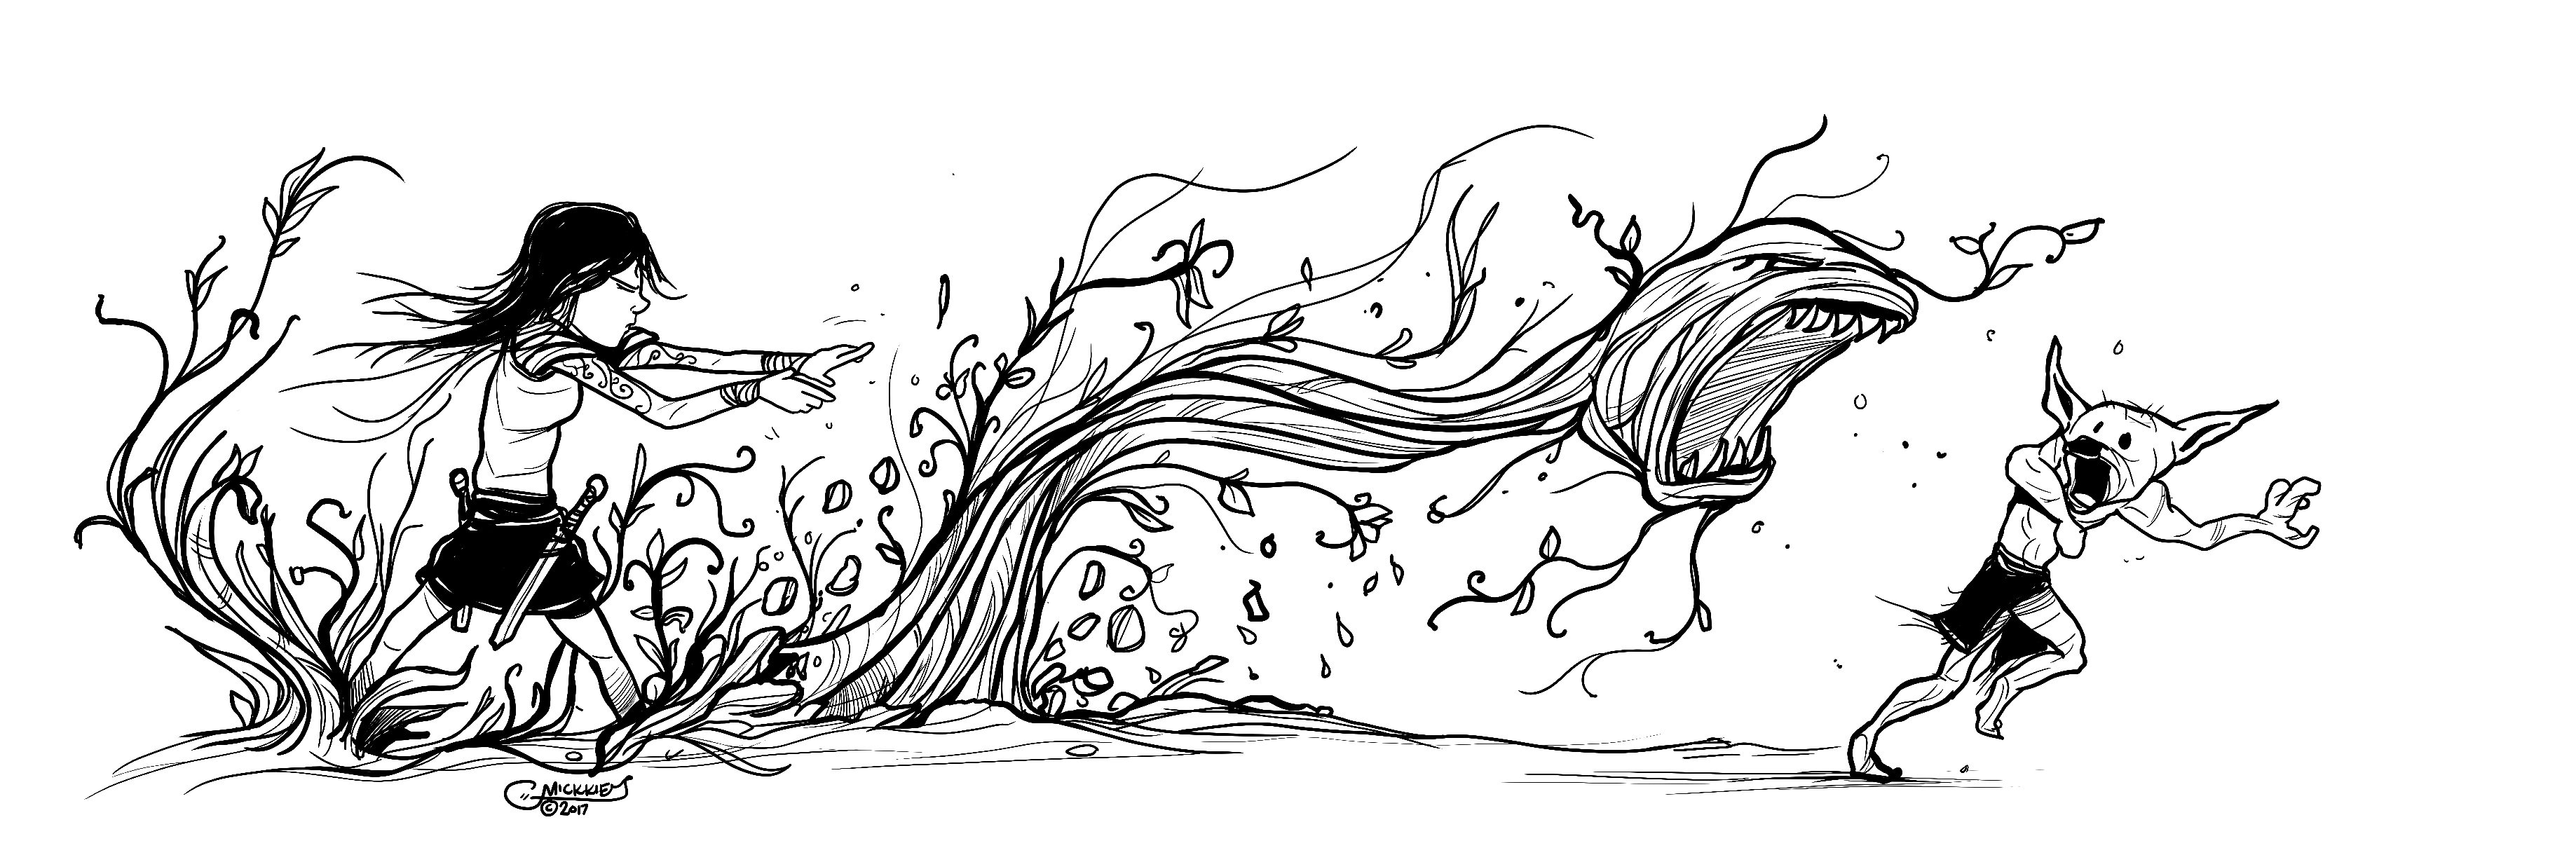
\includegraphics[width=\textwidth]{logo}\\[2cm]
    \vfill
    {\large \today}
\end{titlepage}

\frontmatter  % Begin numbering in Roman numerals

% Table of Contents
\tableofcontents

\mainmatter   % Switch to Arabic numerals for the main part of the book
\setlength{\columnsep}{1cm}  % Space between columns

%%Protože jsou kapitoly dlouhé, je každá jako jeden TeX dokument
\chapter{Úvod}
\label{chap:introduction}
\subfile{chapters/uvod}

\begin{figure}[h!]
  \centering
  \caption{\href{https://davidramos.ca/wp-content/uploads/2021/04/cyn-1024x576.png}{source}}
  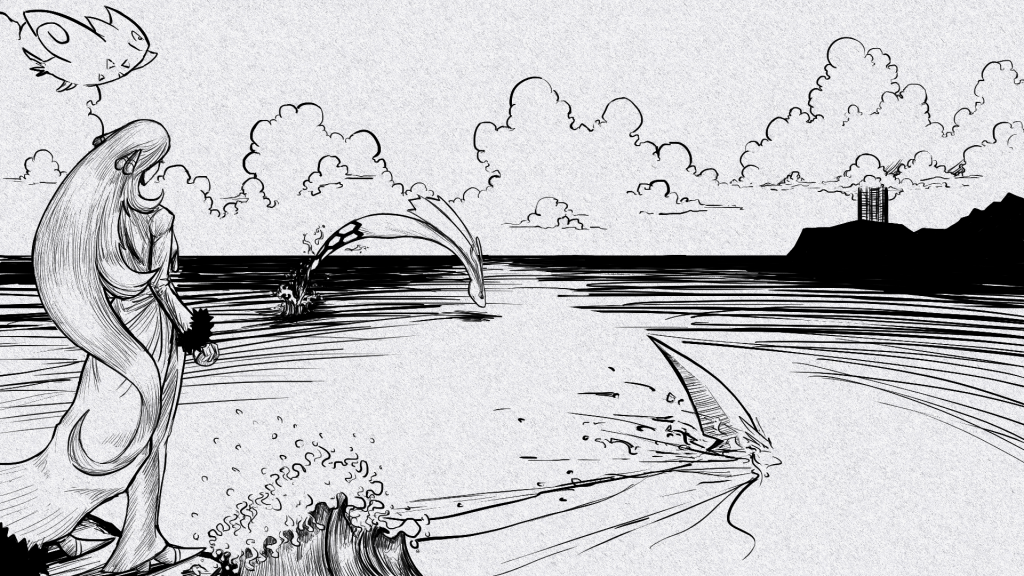
\includegraphics[width=\textwidth]{jezero}
\end{figure}

\chapter{Aspekty a body osudu}
\label{chap:aspekty}
\subfile{chapters/aspekty}

\begin{figure}[h!]
  \centering
  \caption{\href{https://aukceaukci.s3.amazonaws.com/aukceaukci/production/files/2024/02/06/10/15/12/906b839a-538e-4f31-bbcc-131d423cb646/1.webp}{source}}
  \includegraphics[width=\textwidth]{jules}
\end{figure}

\chapter{Akce a výsledky}
\label{chap:akce}
\subfile{chapters/akce}

\begin{figure}[h!]
  \centering
  \caption{\href{https://pbs.twimg.com/media/EGcmJ2vU0AIqTU9?format=jpg&name=large}{source}}
  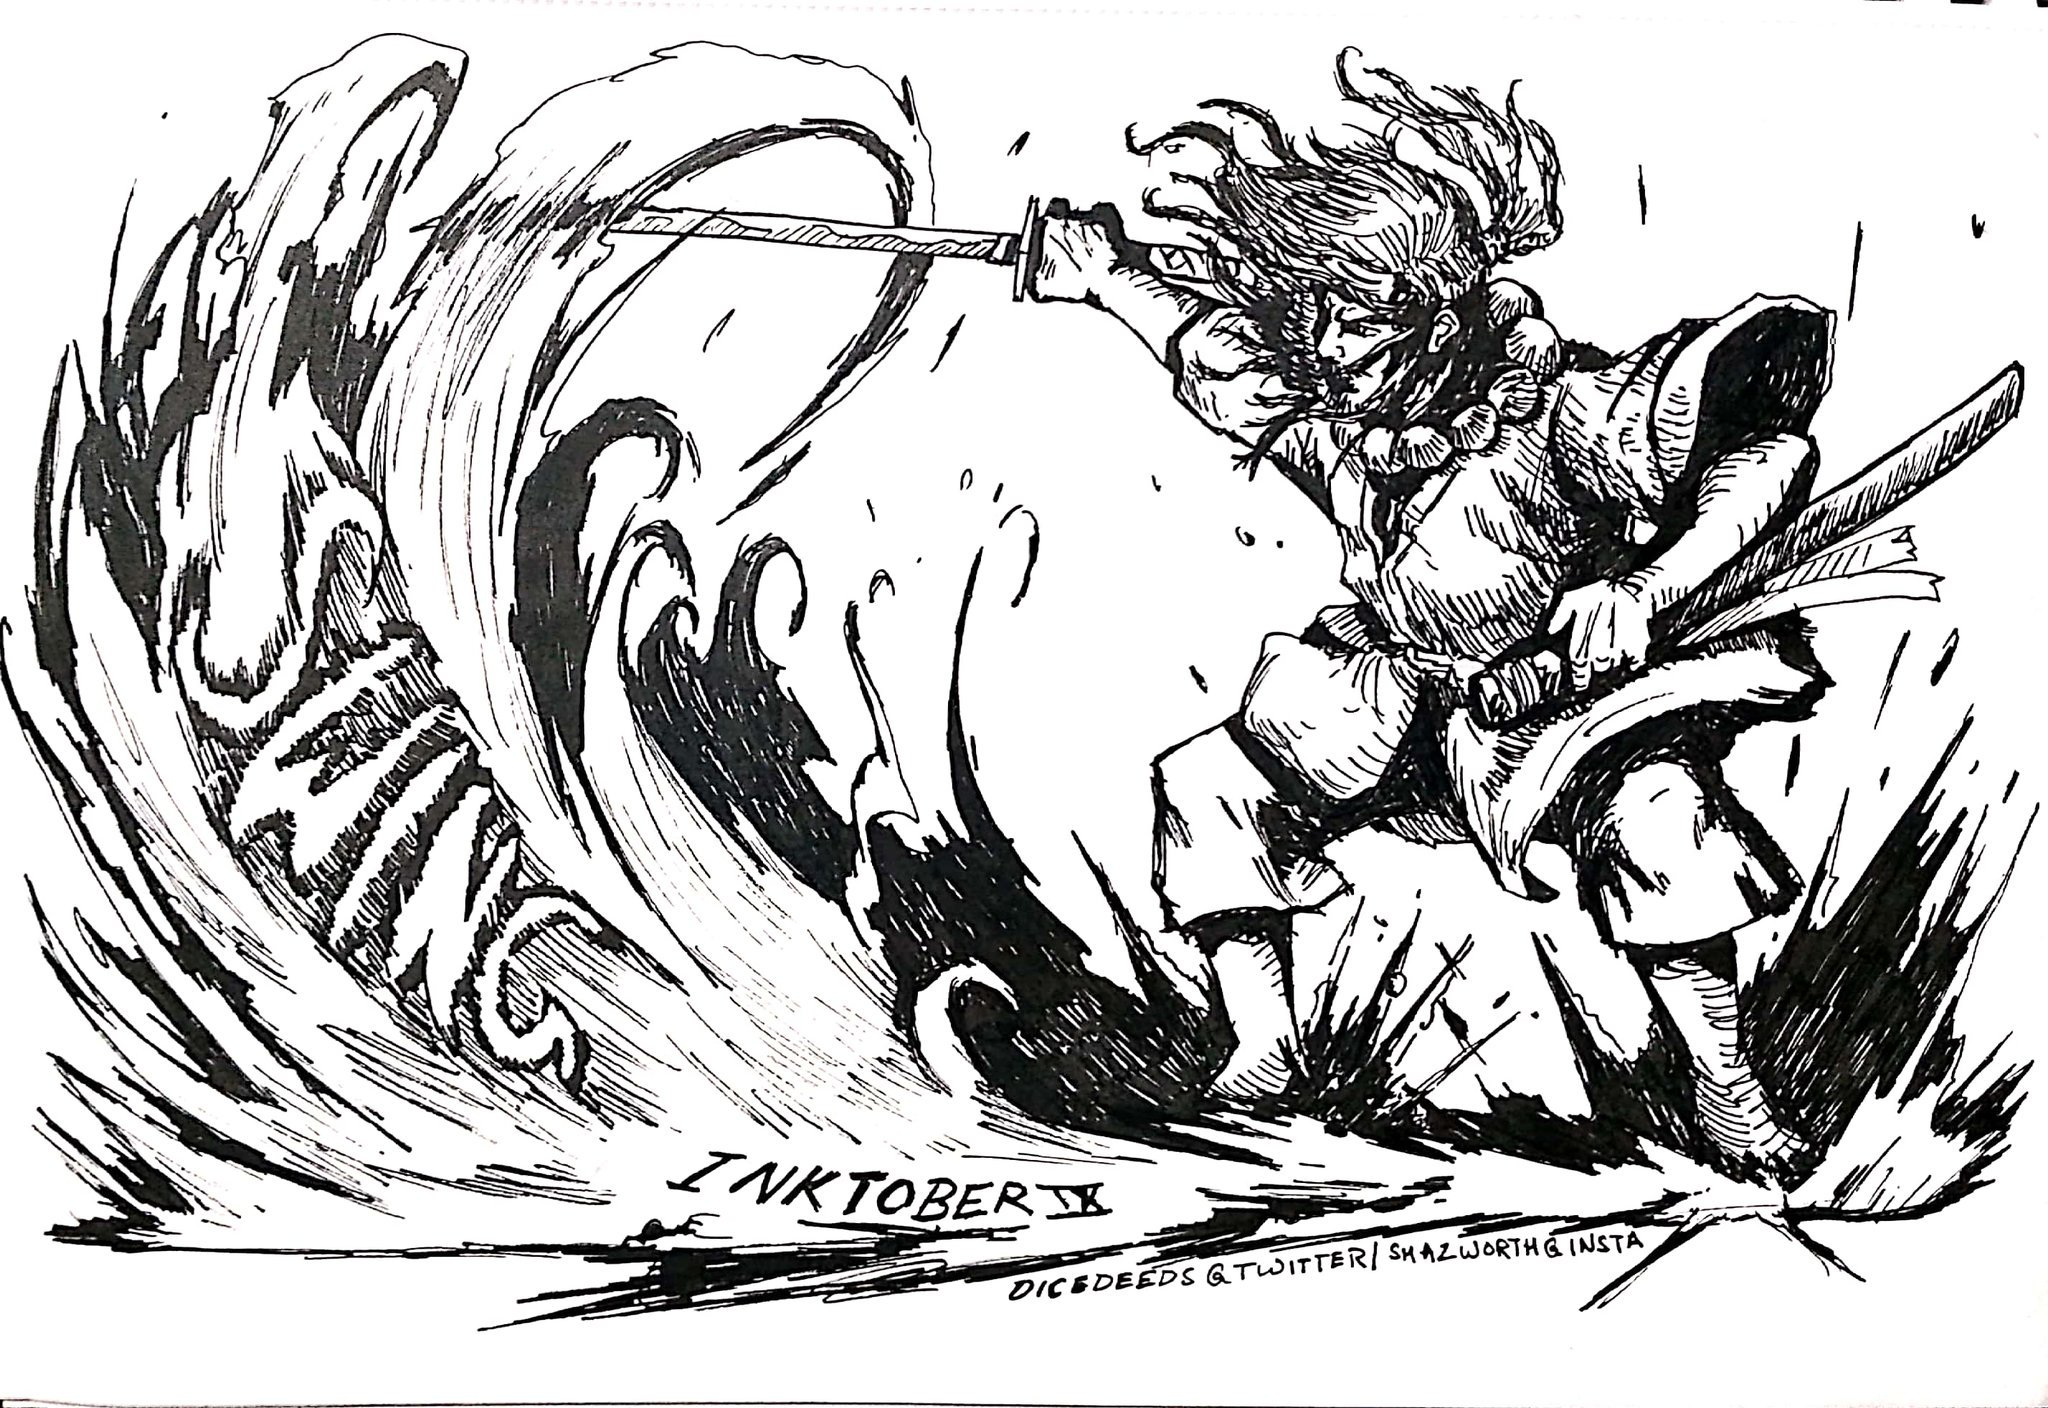
\includegraphics[width=\textwidth]{swing}
\end{figure}

\chapter{Základní dovednosti}
\label{chap:dovednosti}
\subfile{chapters/dovednosti}

\begin{figure}[h!]
  \centering
  \caption{\href{https://www.humanart.cz/user/2527/art/st/2527-1324900216-2.jpg}{source}}
  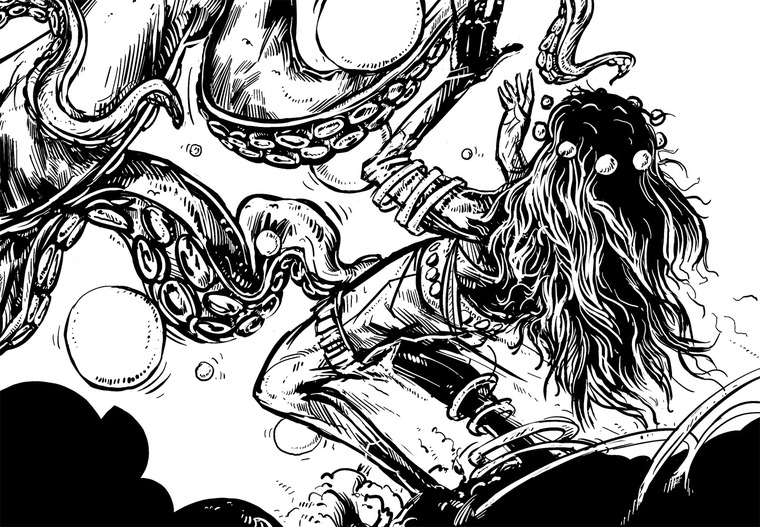
\includegraphics[width=0.75\textwidth]{chobotnice}
\end{figure}

\chapter{Triky}
\label{chap:triky}
\subfile{chapters/triky}

\begin{figure}[h!]
  \centering
  \caption{\href{https://cz.pinterest.com/pin/750623462885443700/}{source}}
  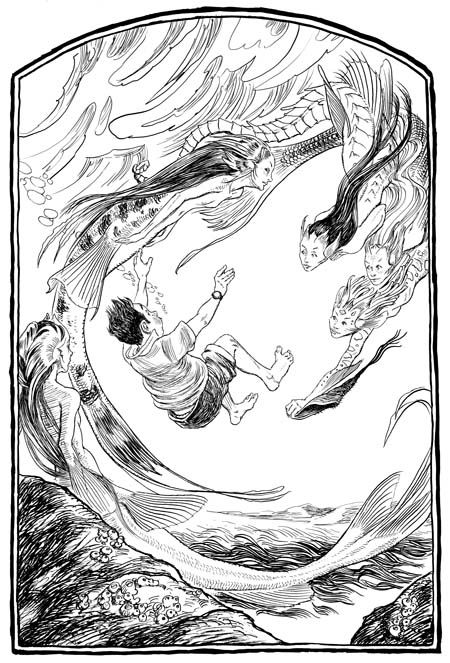
\includegraphics[width=0.75\textwidth]{ryba}
\end{figure}


\chapter{Střety, výzvy a konflikty}
\label{chap:jdesenavec}
\subfile{chapters/strety}

\begin{figure}[h!]
  \centering
  \caption{\href{https://www.pinterest.com/pin/484418503638647556/}{source}}
  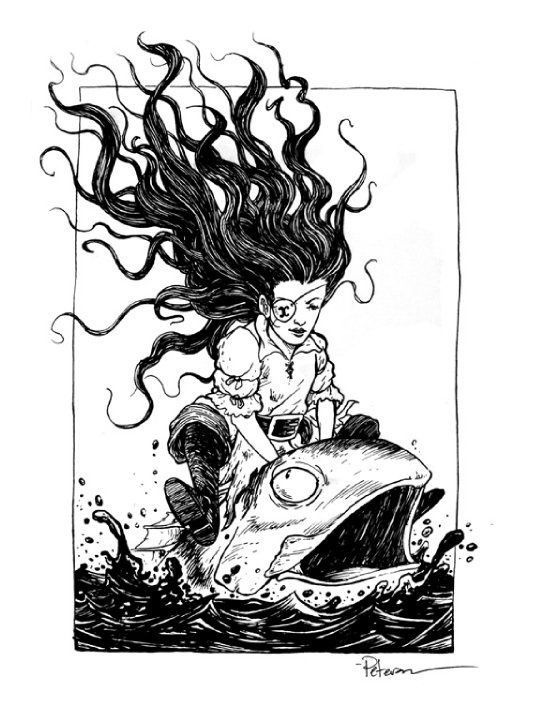
\includegraphics[width=0.5\textwidth]{zaba}
\end{figure}


\chapter{``Povolání''}
\label{chap:speciality}
\subfile{chapters/povolani}

\begin{figure}[h!]
  \centering
  \caption{\href{https://petrakubaskova.cz/wp-content/uploads/2024/07/elixir-cze.png}{source}}
  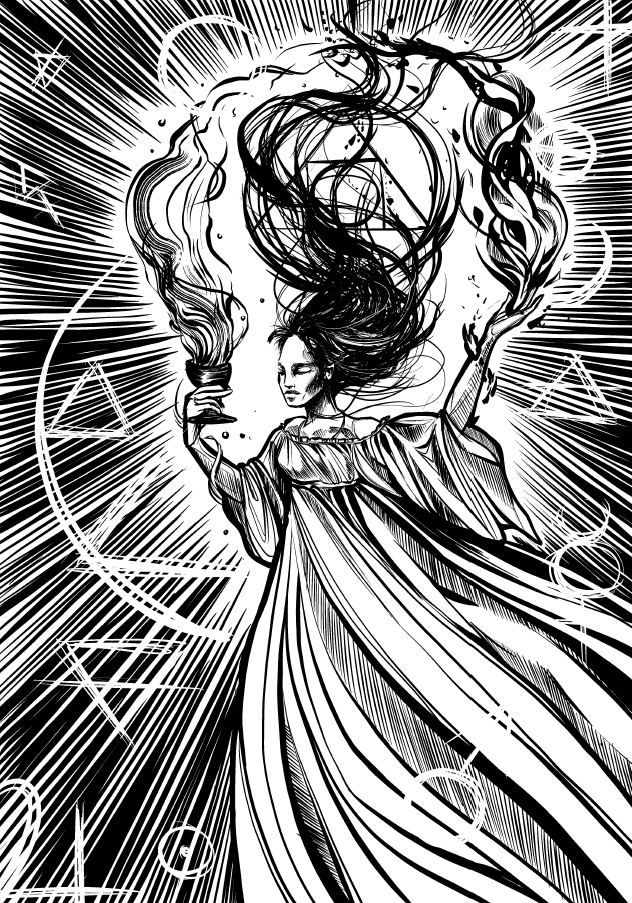
\includegraphics[width=\textwidth]{carodejka}
\end{figure}


\chapter{Magické a speciální předměty}
\label{chap:magicke-spec-predmety}
\subfile{chapters/predmety}


\chapter{Postup a zlepšování postav}
\label{chap:postup}
\subfile{chapters/postup}

\chapter{Dodatky}
\label{chap:dodatky}

\section{K čemu jsou dodatky}
\label{sec:kcemudodatky}

\subfile{chapters/dodatky/uvod}

\section{Sicco}
\label{sec:sicco}

\subfile{chapters/dodatky/sicco}

\section{Netvorobijec}
\label{sec:netvorobijec}

\subfile{chapters/dodatky/netvorobijec}

\section{Edenův bratr}
\label{sec:edenuvbratr}

\subfile{chapters/dodatky/edenuvbratr}

\section{Subotamský mnich}
\label{sec:subatom}

\subfile{chapters/dodatky/subotam}




\end{document}
